\begin{frame}{Les Modèle de Markov Caché(MMC) ou Hidden Markov Model(HMM)}

\begin{block}{Définition}
Un modèle de Markov caché (MMC) est un modèle
statistique permettant de représenter un processus
de Markov dont l’état est non observable. 
	\end{block}
	\begin{block}{Processus markov(Chaîne de Markov)}
	En mathématiques, un processus de Markov est un processus stochastique possédant la propriété de Markov. Dans un tel processus, la prédiction du futur à partir du présent n'est pas rendue plus précise par des éléments d'information concernant le passé.
	\end{block}
\end{frame}


\begin{frame}{Un exemple illustratif de HMM}
\begin{figure}
\centering
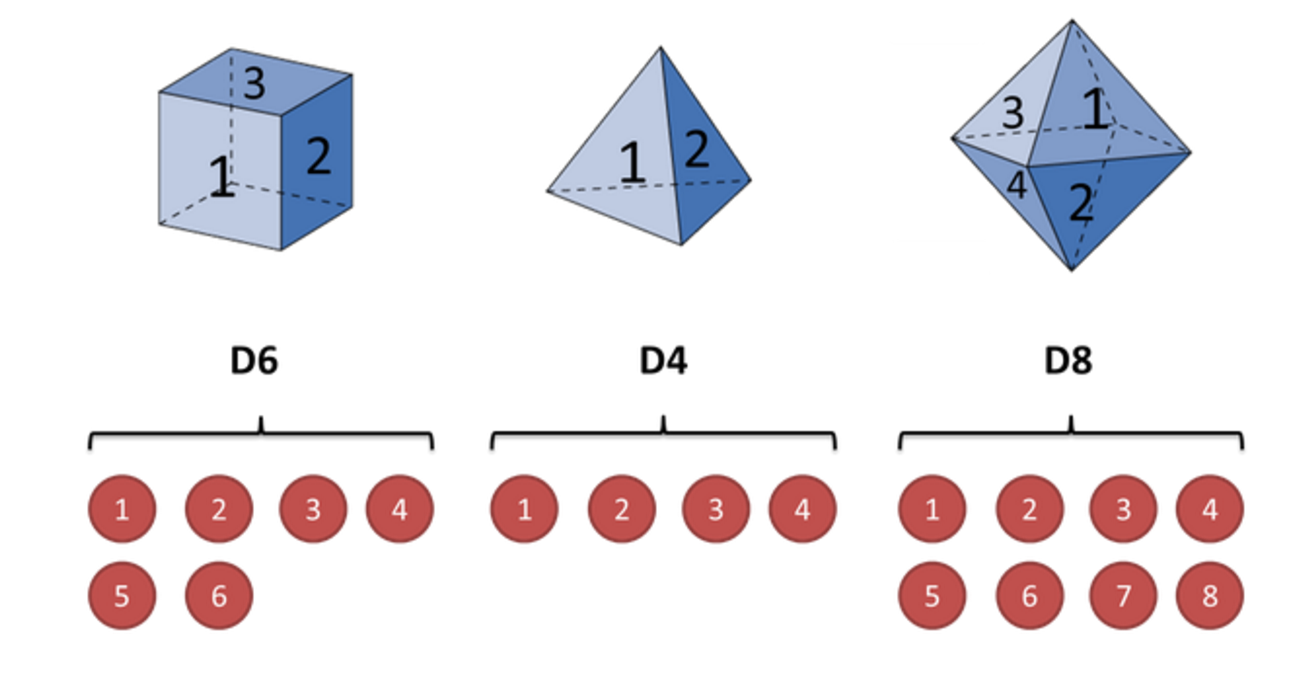
\includegraphics[width=8cm]{images/hmm.png}
\caption{Un exemple de HMM}
\end{figure}
\end{frame}



\begin{frame}{Un exemple illustratif de HMM}

\begin{figure}
\centering
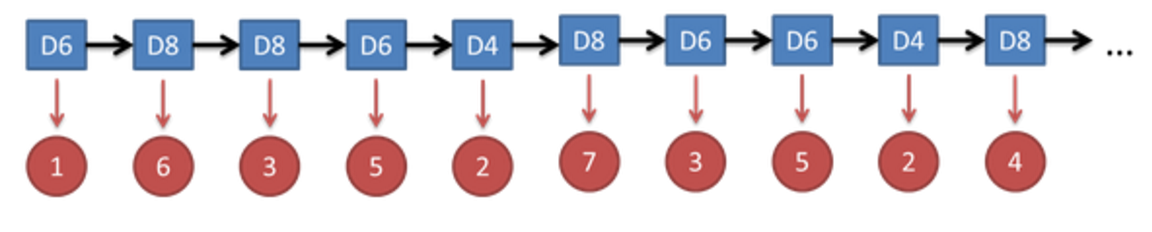
\includegraphics[width=8cm]{images/hmm1.png}
\caption{Un exemple de HMM}
\end{figure}
\begin{itemize}
\item Les états observés : 1 6 3 5 2 7 3 5 2 4
\item Les états cachés : D6 D8 D8 D6 D4 D8 D6 D4 D8
\end{itemize}

\end{frame}

\begin{frame}{Algorithm de Viterbi}

\begin{itemize}
\item L’algorithme de Viterbi permet de calculer
la valeur la plus probable des états cachés du processus
étant donneê des données observables. 
\end{itemize}

\end{frame}

\begin{frame}{Modèle acoustique}

	
\end{frame}